%Using a UAV for Destructive Surveys of Mosquito Population
\chapter[UAV Surveying Mosquitoes]{Using a UAV for Destructive Surveys of Mosquito Population}

This chapter presents research performed for the ICRA paper "Using a UAV for Destructive Surveys of Mosquito Population", by A. Nguyen, D. Krupke, M. Burbage, S. Bhatnagar, S.P. Fekete, and A.T. Becker.

I constructed the UAV and the attachment of the net, as well as assisted in early generations of the net. I piloted all UAV test and programmed the autonomous tests of our algorithm and data collection. I also designed the method to measure powerconsumption of the UAV and analyzed the data.

\section[RelatedWork]{Overview and Related Work}
%%%%%%%%%%%%%%%%%%%%%%%%%%%  

\noindent  \emph{Mosquito Control Solutions}:
Mosquito control also has a long history of efforts associated both with monitoring mosquito populations~\cite{dennett2007associations} and with eliminating mosquitoes.
The work involves both draining potential breeding grounds and destroying living mosquitoes~\cite{peter2005tick}.
An array of insecticidal compounds has been used with different application methods, concentrations, and quantities, including both larvicides and compounds directed at adult mosquitoes~\cite{larvicides2005guidelines}.

Various traps have been designed to capture and/or kill mosquitoes with increasing sophistication in imitating human bait, as designers strive to achieve a trap that can rival the attraction of a live human~\cite{maliti2015development}.
In recent history, methods have also included genetically modifying mosquitoes so that they either cannot reproduce effectively or cannot transmit diseases successfully~\cite{marshall2009malaria}, and with the recent genomic mapping of mosquito species, new ideas for more targeted work have been formulated~\cite{hill2005arthropod}.

Popular methods to control mosquitoes such as insecticides are effective, but they have the potential to introduce long-term environmental damage and mosquitoes have demonstrated the ability to become resistant to pesticides~\cite{ndiath2012resistance}.
Traditional electrified screens (bug zappers) use UV light to attract pests but have a large bycatch of non-pest insects~\cite{University-Of-Florida1997}
This chapter introduces techniques using bug zappers mounted on unmanned vehicles to autonomously seek out and eliminate mosquitoes in their breeding grounds and swarms.
Instrumentation on the bug zappers logs the GPS location, altitude, weather details, and time of each mosquito hit.
Mosquito control offices can use this information to analyze the insects' activities.
The device can be mounted on a remote-controlled or autonomous unmanned vehicle.
If autonomous, the vehicle can use the data collected from the electrified screen as feedback to improve the effectiveness of the motion plan. 
	
\noindent  \emph{Robotic Pest Management}:
As GPS technology has flourished and data processing has become cheaper and more readily available, researchers have explored options for implementing the new technologies in breeding ground removal~\cite{anupa2014identification} and more effective insecticide dispersion~\cite{hur2015low}.  Low-cost UAVs for residential spraying are under development~\cite{amenyo2014medizdroids}.  Even optical solutions have been considered, including laser containment~\cite{boonsri2012laser} or, by extension, exclusion and laser tracking and extermination~\cite{kare2010build}.
    
\noindent \emph{Robotic Coverage}: 
Robotic coverage has a long history. The basic problem is one of designing a path for a robot that ensures the robot visits within $r$ distance of every point on the workspace.  For an overview see~\cite{Choset2001}.  This work has been extended to use multiple coverage robots in a variety of ways, including using simple behaviors for the robots~\cite{spears2006physics,Koenig2001}.

\section[Hardware Design]{Hardware Design}
%%%%%%%%%%%%%%%%%%%%%%%%%%%%%%%%%%%%%%%

This section examines the components of the mosquito UAV system, shown in Fig.~\ref{fig:DroneAndNet}. This includes the UAV, electrified screen, surveying electronics, and a discussion of the energy budget. 
%The design for the mosquito UAV system been assigned a U.S.\ Provisional Patent Application~\cite{Becker2016patentapp}.

\subsection{The UAV}

The UAV is a custom-built, $\SI{177}{\centi\metre}$ wingspan hexacopter, controlled by a Pixhawk flight controller running ArduPilot Mega flight software. The UAV has a 3DR GPS module using the UBlox NEO-7 chipset.

\subsection{Screen Design}
The mosquito screen is designed to eliminate high density mosquito populations. 
This screen was constructed from two expanded aluminum mesh panels, spaced apart by \SI{3}{\milli\metre} thick ABS grid. 
These mesh panels have \SI{12}{\milli\metre} diamond-shaped  openings, and is held taught by nylon bolts around the perimeter.  
The bottom mesh panel is offset by half a diamond (6 mm) to the right to ensure all insects greater than 6 mm cannot pass through the net.
The top mesh is held at the reference voltage and the bottom mesh is energized to $1.8~kV$ above the reference voltage.

The perimeter is reinforced by two sets of \SI{7}{\milli\metre} diameter fiberglass rods that are inset into 3D printed corner fixtures.
These rods protect the frame from getting damaged from any side, and allows the UAV to land without damaging the net.


Once assembled, the net weighs \SI{0.948}{\kilogram} and has an overall area of \SI{0.194}{\square\metre}, with the spacer occupying \SI{0.0325}{\square\metre}. 
This makes the effective net area \SI{0.161}{\square\metre}. %, and the total cost of building a net this size is only \$27.44 USD.



%Design files and build instructions are available at~\cite{Vinh2016BugNet}.


%%%%%%%%%%%%%%%%%%%%%%%
\subsection{Screen Location}
The UAV carries the bug-zapping screen, which is suspended by paracord rope at each corner.  The location of this screen determines the efficacy of the mosquito UAV, measured in mosquitoes detected per second of flight time. The following describes a simplified analysis to optimize the screen location.

For manufacturing ease, the electrified screen is a rectangle with a width of $d_s$. The screen is suspended a distance $h_s$ beneath the UAV flying at height $h_d$.  We chose to suspend the screen beneath the UAV to avoid the weight of the rigid frame that would be required if the screen were above the UAV and because most mosquito species prefer low flight~\cite{gillies1976vertical}.  This screen can be suspended at any desired angle $\theta$ in comparison to horizontal, as shown in Fig.~\ref{fig:DroneConfigs}.
Two key parameters are the distance $h_s$ and the optimal angle $\theta$.  The goal is to clear the greatest volume of mosquitoes per second, a volume defined by the UAV forward velocity $v_f$ and the cross-sectional area $h_m \times d_s$ cleared by the screen, as shown in Fig.~\ref{fig:AngleVsSpeed}.

To hover, the UAV must push sufficient air down with velocity $v_d$ to apply a force that cancels the pull of gravity.  The UAV and screen combined have mass $m_{d}$ and its cross section can be approximated as a square with a side length of $d_d$.  The mass flow of air through the UAV's propellers is equal to the product of the change in velocity of the air, the density of the air $\rho_a$, and the cross sectional area.

\begin{figure}
\centering
\begin{overpic}[width=\columnwidth]{icra2018/DroneConfigs.pdf}\end{overpic}
\caption{\label{fig:DroneConfigs}
The UAV suspends a rectangular bug-zapping screen beneath it.  Propwash pushes incoming mosquitoes downwards, and the UAV clears a volume $h_m \times d_s \times v_f$ each second. Circles show two mosquitoes at equal time intervals relative to the UAV.} 
\vspace{-1em}
\end{figure}


We assume that air above the UAV is quiescent, so the change in velocity of the air is $v_d~ \si{\metre\per\second}$. So that 
\begin{align} \label{eq:forceBalanceForDrone}
\text{Force gravity} & = \left(\text{mass flow}\right) \cdot \text{air velocity and } \nonumber \\
m_{d} \cdot  g &= (v_d \cdot  \rho_a \cdot  d_d^2 ) \cdot  v_d. 
\end{align}

Then the required \emph{propwash}, the velocity of air beneath the UAV, for hovering is
\begin{align} \label{eq:dronePropwash}
v_d = \sqrt{ \frac{ m_d g}{\rho_a d_d^2} }.
\end{align}
The flight testing site in Houston, Texas is \SI{15}{\metre} above sea level. At sea level the density of air $\rho_a$ is \SI{1.225}{\kilogram\per\cubic\metre}.
The UAV and instrumentation combined weigh \SI{5.1}{\kilogram} with a width of \SI{0.75}{\metre}. The acceleration due to gravity is \SI{9.871}{\metre\per\square\second}.  Substituting these values gives $v_d = \SI{8.5}{\metre\per\second}$.

Due to propwash, an initially hovering mosquito will fall when under the UAV at a rate of $v_d$.  Relative to the UAV, the mosquito moves horizontally at a rate of $-v_f$.  As shown in Fig.~\ref{fig:DroneConfigs}, we can extend lines with slope $-v_d/v_f$ from the screen's trailing edge to $h_{\textrm{top}}$ and from the leading edge to $h_{\textrm{bottom}}$.
\begin{align} \label{eq:ClearedCrossSection}
h_{\textrm{top}} &= h_d - h_s + \frac{d_s}{2} \sin(\theta) +  \frac{d_d + d_s\cos(\theta)}{2}  \frac{v_d}{v_f} \nonumber \\
h_{\textrm{bottom}} &= h_d - h_s - \frac{d_s}{2} \sin(\theta) +  \frac{d_d - d_s\cos(\theta)}{2}  \frac{v_d}{v_f}  \nonumber \\
h_m &= h_{\textrm{top}} - h_{\textrm{bottom}} =  d_s\left(\frac{v_d}{v_f}\cos(\theta) + \sin(\theta) \right)
\end{align}
The optimal angle is therefore a function of forward and propwash velocity:
\begin{align} \label{eq:OptimalScreenAngle}
\ \theta = \mathrm{ArcTan}\left(\frac{v_f}{v_d}\right).
\end{align}

To ensure the maximum number of mosquitoes are collected, the screen must be sufficiently far below the UAV $ h_s > \frac{d_s}{2} \sin(\theta) +  \frac{d_d + d_s\cos(\theta)}{2}  \frac{v_d}{v_f}$  and the bottom of the screen must not touch the ground, $ h_d > h_s + \frac{d_s}{2} \sin(\theta) $.

\begin{figure}
\centering
\begin{overpic}[width=\columnwidth]{icra2018/AngleVsSpeed.pdf}\end{overpic}
\caption{\label{fig:AngleVsSpeed}
The volume cleared by a UAV is a function of screen angle $\theta$ and forward velocity $v_f$.  Dotted line shows the optimal angle given in \eqref{eq:OptimalScreenAngle}. } 
\vspace{-1em}
\end{figure}

There are practical limits to $h_s$ as well.  Tests with $h_s > \SI{2}{\metre}$ were abandoned because the long length caused the screen to act as a pendulum, introducing dynamics that made the system difficult to fly.

Changing the flying height $h_d$ of the UAV will target different mosquito populations because mosquitoes are not distributed uniformly vertically. 
Gillies and Wilkes demonstrated that different species of mosquitoes prefer to fly at different heights~\cite{gillies1976vertical}. 

%%%%%%%%%%%%%%%%%%%%%%%
\subsection{Wind Tunnel Verification of Net Angle}

This section describes experiments run in a wind tunnel to verify the simplified net angle analysis in the previous section. 
Smoke streaklines were used to visualize the flow of air as it passed by the UAV.
Due to space constraints in the wind tunnel, a free-flying phantom 4 was used instead of the hexacopter used for carrying the zapper. 
The wind tunnel was set to a \SI{3}{\metre\per\second} flow speed, and the UAV manually flown in approximately stable hovering.
The solo UAV is \num{0.3} $\times$ \num{0.3} $\times$ \SI{0.2}{\metre}.  The windtunnel has a \SI{1}{\metre} $\times$ \SI{1}{\metre} cross section. 
%??? brand name of the smoking apparatus?
As seen from Fig.~\ref{fig:WindTunnel}, the proposed screen position captures free flowing air and air entrained by the UAV propellers.
This test encouraged us to mount the net as close to the UAV as possible, so that air, and flying mosquitos, entrained by the propellers are pushed into the net.


\begin{figure}
\centering
\begin{overpic}[width=1.0\columnwidth]{icra2018/WindTunnelv01lowres.pdf}\end{overpic}
\caption{\label{fig:WindTunnel}
	Frames from wind tunnel test with free-flying UAV at \SI{3}{\metre\per\second} windspeed with smoke for streaklines~\cite{Bhatnagar2018}.  As shown in the frames at right, the proposed screen position (in red) captures free flowing air and air entrained by the UAV propellers.
	Each black square is \SI{25.4}{\milli\metre} in width.
} \vspace{-1em}
\end{figure}


%%%%%%%%%%%%%%%%%%%%%%%
\subsection{Data Logger}

The electrical detection and logging system is powered by a $9~V$ lithium ion battery applied directly to the controller and two AA $3~V$ lithium ion batteries applied to the power circuit for the screen.
The controller uses a GPS shield for monitoring the location and altitude as well as a real time clock to timestamp each data point collected from the system.
A Raspberry Pi 3 is used for data logging, 
sensors include a GPS sensor (NEO-6M Ublox), 
a capacitive humidity sensor, a thermistor (DHT22),
%ADS1115 16-bit ADC for monitoring the supply-side voltage of the net, and 
and an INA219 high side, 12-bit DC current sensor for monitoring the supply-side current delivered to the net.
The net current draw is logged at 100 Hz, while GPS and weather sensor data is logged at 1Hz.  
All data is stored on an onboard SD card.

%%%%%%%%%%%%%%%%%%%%%%%
\subsection{Energy Budget}

\begin{figure}
\centering
\begin{overpic}[width=0.9\columnwidth]{icra2018/OscilloscopeTrace.pdf}\end{overpic}
\caption{\label{fig:BugZapTrace}
					  Current, voltage, and power traces for five \textit{Culex quinquefasciatus} mosquitoes as each contacts the bug-zapping screen at $t=0$.  Contact causes a brief short that recovers in $\SI{160}{\milli\second}$.
} 
\vspace{-1em}
\end{figure}
% \todo{what is the new energy usage of the screen?}


Tests with an oscilloscope show that in the steady state, a $\SI{30.5}{\centi\metre} \times \SI{61}{\centi\metre}$ screen and electronics have a power consumption of \SI{3.6}{\watt}.  During a zap, the screen voltage monitoring circuit shorts briefly when the mosquito contacts the screen.  Figure~\ref{fig:BugZapTrace} shows the time sequences for battery and screen voltages, current, and power during five mosquito zaps.  
% % WE COULD NOT JUSTIFY THIS EQUATION 
%%  The initial current spike recovery can be modeled with an exponential fit.
%%
% \begin{align} \label{eq:BugZapFit}
%i=69.1e^{-2.7\times10^4 t} ~A
%\end{align}
%%
%The fit in \eqref{eq:BugZapFit} gives a time constant of $36~\mu s$ for the short and a recovery time of $80~\mu s$. 
Multiplying voltage by current to find the instantaneous power ($p=iv$) and integrating the area under the power curve show a total energy consumption of \SI{4.2}{\milli\joule} for each zap.  Recharging the screen requires more power and is represented in the latter part of the curves.  The overall recovery time is about $\SI{160}{\milli\second}$.  Most of the energy is consumed charging and maintaining the charge on the screen rather than in zapping the mosquitoes.





%Data
%The files used for this run of simulations are as follows:
%MosquitoFlightSimv2p0.m
%MosquitoSimv2p2randombounce.m
%MosquitoSimv2p2boustrophedon.m
%MosquitoSimComparev1p0.m
%
%All are located in the Dropbox code folder.
%Raw data are located in the Excel file Simulation Results.xlsx.
%    

%%%%%%%%%%%%%%%%%%%%%%%%%%%%%%%%%%%%%% 
\section[Path Planning]{Planning minimal turn cost paths}
%%%%%%%%%%%%%%%%%%%%%%%%%%%%%  

\newcommand{\revised}[1]{{\color{red}#1}}

%The following section present an overview of the algorithm used in the paper's research, which was done by our collaborators in Germany:
%D. Krupke and S.P. Fekete of TU Braunsweig.

\subsection{Modelling mosquito density}
\label{subsec:modelling}
Due to a-priori knowledge of mosquitos' preferred habitats from entomology, we can model the density of mosqitos in a field we want to cover.
This knowledge will help us plan the most efficient path, killing the most mosquitos with the least amount of energy used.
First, we divide a field for coverage into a pixel grid, the size of each pixel dictated by the size of the net and the resoultion of the UAV's GPS.
Each pixel $p_i\in P$ we give a relative density value $c(p_i)$ that describes the estimated mosquito density based on the environmental factor of the pixel.
In $P$ there will only be a subet with high relative density value.
The goal is to maximize the density covered by the set $S\subseteq P$ of visited pixels i.e., $\max_{S\subseteq P} \sum_{p_i\in S} c(p_i)$ within the available battery capacity.
This could be done in one single trip or over multiple trips with multiple batteries.

%The data on the distribution of mosquitoes is given for a two-dimensional grid environment; the grid size
%is induced by the size of the screen, the available data and the desired resolution of the extracted map. 
%For each pixel $p_i\in P$, we are given a relative value
%$c(p_i)$ that describes the estimated a-priori density of mosquitoes, based on data obtained from boustrophedon (back and forth) scans of the area by the UAV;
%this implies that only a subset of pixels carry a significant value.
%Visiting one of the pixels corresponds to sampling and mapping the actual density distribution of mosquitoes. 
%For a dense distribution of mosquitoes
%(which is the case for the instances relevant for pest control), multiple visits to the same pixel do not contribute additional
%knowledge. As a consequence, the objective is to maximize the sampling value of the set $S\subseteq P$ of visited pixels, 
%i.e., $\max_{S\subseteq P} \sum_{p_i\in S} c(p_i)$ {within the available battery capacity}; this may be over the course of a single closed trajectory, or over
%a combination of multiple roundtrips. 

\subsection{Turn cost}

\begin{figure}[h]
\begin{center}
\includegraphics[width=.75\columnwidth]{icra2018/turncost}
\caption[Mosquito hunting drone]{Turns are expensive. See our related video at
\url{https://youtu.be/SFyOMDgdNao} for details, and
\cite{becker2017zapping} for an accompanying abstract.} \label{fig:turncost}
\end{center}
\vspace{-1em}
\end{figure}

UAVs can make turns on the spot, without curvature constraints like a fix-winged aircraft.
However, UAVs turns are energtically expensive.
As Fig.~\ref{fig:turncost} shows, the energy required per meter of travel in a turn is 4 to 5 times as expensive as traveling through a straight path.
The limiting factor for a UAV's flight is its battery capacity, therefor it is important to limit the amount of turns needed per flight while maximizing the amount of pixels visited.
To consider the total energy cost of a turn, we need to limit the types of turns the UAV made.
We consider only strict set of \ang{90} and \ang{180} turns since the UAV does not have minimal turn curvature.
Additionally, the two turn angles allow us to fly around most large obstacles while visiting the pixels around it.

%Planning good trajectories for a UAV is not subject to the same curvature constraints of an ordinary aircraft
%because UAVs can turn on the spot. However, turns are a critical aspect of path
%planning due to their impact on energy consumption.  Battery capacity is {\em the} limiting factor for  UAV flight time. As shown in Fig.~\ref{fig:turncost}, 
%the power output for a desired trajectory is non-uniform.  Flying along a straight path
%is relatively inexpensive but turning is energy intensive. 

%As a consequence, we must consider the total turn costs associated
%with changing direction, as measured by the turn angle.
%As we are not limited by trajectory curvature, we refer to straight-line connections and a finite set of $2\omega$ different
%headings for visiting vertices. For the most natural case of orthogonal grids $\omega=2$. When
%surveying non-isolated mosquito hotspots (whose size greatly exceeds the size of the UAV), we are not dealing with
%isolated pixels and the modeling error of this restriction is small.

%TODO: I guess one can save space here by e.g. skipping subset cover.
%Now we consider different trajectory types.
%A {\em cycle} is a roundtrip of a subset $S\subseteq P$ that visits all points in $S$ and returns to the origin, a {\em cycle cover} of $P$ is a set of cycles
%that together visit all points in $P$, and a {\em tour} is a single cycle that visits all points in $P$. A {\em subset cycle cover} for $S\subset P$ is a cycle
%cover that covers at least the points in $S$, while a {\em subset tour} is a tour of at least the points in $S$. For any of these structures, we are interested in
%%cycle covers or tours of {\em minimum total turn cost}. 
%{cycle covers or tours of {\em minimum total travel cost}. 
%The travel/battery cost is a linear combination of the number of pixel transitions (distance) and the weighted number of turns, 
%corresponding to the total turn angle.
%}
%In addition, a {\em minimum turn-cost penalty cycle cover}  or a {\em minimum turn-cost penalty tour}
%visits a subset $R\subset P$, such that the sum of total travel cost and the sum $\sum_{i\not\in R} c(p_i)$ of values of 
%unvisited pixels is minimized. 
%The travel/battery cost is a linear combination of the number of pixel transitions (distance) and the weighted number of turns, 
%corresponding to the total turn angle.
%Note that the travel cost
%may be a linear combination of turn and travel cost, as long as triangle inequality is satisfied.

%\subsection{Computational Complexity}
%\label{subsec:complexity}
%Finding optimal covering paths that map a given region is closely related to the famous 
%\emph{Traveling Salesman Problem (TSP)}, which asks to minimize
%total length of a single tour that covers all of a given set of locations. The TSP is one of 
%the classic NP-hard problems, so we cannot expect a general method that finds
%a provably optimal solution for any  instance in polynomially bounded time.
%A generalization of the TSP is
%the \emph{Lawnmower Problem} (see Arkin et al.~\cite{arkin2000approximation}, which considers coverage by
%a tool of nontrivial size. For the objective of minimizing the total cost (in particular, the turn
%cost), Arkin et al.~\cite{arkin2005optimal} showed that finding minimum-turn tours in grid graphs is NP-hard,
%even if a minimum-turn cycle cover is given. The complexity of finding a set of multiple cycles that cover a 
%given set of locations at minimum total turn cost had remained elusive for many years; \emph{Problem~{53}} in \emph{The Open Problems Project}
%%edited by Demaine, Mitchell, and O'Rourke~\cite{openproblemproject}
%asks for the complexity of finding a minimum-cost (full) cycle cover in a 2-dimensional grid graph. This is not 
%obvious: large parts of a solution can usually easily be deduced by local information and 2-factor techniques.
%Arkin et al. showed~\cite{arkin2005optimal,arkin2001optimal} that the full coverage variant in {\em thin} grid graphs (which do not contain a $2\times 2$ square,
%so every pixel is a boundary pixel) is solvable in polynomial time. In separate work~\cite{dom3}, two of us were able to resolve this
%issue by showing that finding a cycle cover of minimum turn cost is  NP-hard.

%\subsection{Mathematical Optimization}
%\label{subsec:complexity}
%A powerful approach for finding optimal solutions to instances of NP-hard problems is the use
%of Integer Programming (IP). While solving an IP still requires exponential time in the worst case,
%using carefully crafted mathematical models in combination with specific algorithm engineering and available
%IP solvers enables solving instances of considerable size to provable optimality.
%For our purposes, we can describe the problem as follows. 
%
%\paragraph{Penalty Cycle Covers}
%The set $P$ of pixels corresponds to a given grid graph $G(P,E)$ in which each pixel $p_j\in P$ is adjacent to the set $N(p_j)$
%of pixels in $P$ that share an edge with $p_j$.
%Each vertex $p_j\in P$ has a scalar reward $c(p_j)$ for visiting (or penalty for not visiting), 
%and a function $\text{cost}_j(i,k)\in \mathbb{Z}^+_0$  that maps the cost of traveling from $p_i$ to $p_j$ to $p_k$, where  $p_i,p_k\in N(p_j)$ are adjacent pixels to   $p_j$.
%This cost is symmetric, i.e. $\text{cost}_j(i,k)=\text{cost}_j(k,i)$. %TODO: Or cost(ijk) or cost(i,j,k) or cost(p_i, p_j, p_k)
%The integer program uses two types of variables: integer variables
%$x_{ijk}=x_{kji}$ that state how often passage $p_i-p_j-p_k$ or $p_k-p_j-p_i$ is used and
%Boolean variables $y_{j}$ that indicate that the pixel $p_j\in V$ is not covered,
%i.e., the penalty is paid.  This results in the following formulation: 
%%IP Formulation TODO
%%\begin{strip}
%%\begin{eqnarray}
%%	\min & \displaystyle  \sum_{p_j\in P} \sum_{p_i,p_k\in N(p_j)} \text{cost}_j(i,k) \cdot x_{ijk} + \sum_{p_j\in P}c(p_j) \cdot y_j\label{eq:obj}\\
%%	\text{s.t.}			& 1\leq\displaystyle 4 \cdot y_j +\sum_{p_i,p_k\in N(p_j)} x_{ijk} \leq 4&\forall p_j\in P \label{eq:ip:constr1}\\
%%						& \displaystyle 2 \cdot x_{jij} +\sum_{p_k\in N(p_i), p_k\not= p_j}x_{jik} = 2 \cdot x_{iji}+\sum_{p_k\in N(p_j), p_k\not= p_i}x_{ijk}  & \forall \{p_i,p_j\}\in E \label{eq:ip:constr2}\\
%%						& x_{ijk}\in\mathbb{N}_0, y_j\in \mathbb{B} & \forall p_j\in P, \{p_i,p_k\}\subseteq N(p_j)
%%\end{eqnarray}
%%\end{strip}
%\begin{eqnarray}
%	\min  \displaystyle  \sum_{p_j\in P} \sum_{p_i,p_k\in N(p_j)} \text{cost}_j(i,k) \cdot x_{ijk} + \sum_{p_j\in P}c(p_j) \cdot y_j\label{eq:obj}
%\end{eqnarray}
%with constraints
%\begin{eqnarray}
%	 1\leq\displaystyle 4 \cdot y_j +\sum_{p_i,p_k\in N(p_j)} x_{ijk} \leq 4, &\forall p_j\in P \label{eq:ip:constr1}
%\end{eqnarray}
%\begin{eqnarray}	
%%	\displaystyle  x_{jij}   \underset{ p_k\in N(p_i), p_k\not = p_j}{+ \tfrac{1}{2}\sum x_{jik}}  \!\!    =   x_{iji}      \underset{p_k\in N(p_j), p_k\not= p_i}{+ \tfrac{1}{2}\sum x_{ijk}},  & \forall \{p_i,p_j\}\in E 
%	\displaystyle 2 x_{jij}  \!\!\!   \underset{ p_k\in N(p_i), p_k\not = p_j}{+\sum x_{jik}}  \!\!\!\!\!    = 2  x_{iji} \!\!\!     \underset{p_k\in N(p_j), p_k\not= p_i}{+\sum x_{ijk}},  & \forall \{p_i,p_j\}\in E \label{eq:ip:constr2}
%\end{eqnarray}
%\begin{eqnarray}	
%	 x_{ijk}\in\mathbb{N}_0, y_j\in \mathbb{B} ,& \forall p_j\in P, \{p_i,p_k\}\subseteq N(p_j)  \label{eq:ip:constrINTS}
%\end{eqnarray}
%
%
%%Describe IP
%The objective function in Eq.~\ref{eq:obj} minimizes the total cost of the cycles and the uncovered pixels.
%Eq.~\ref{eq:ip:constr1} enforces a pixel to be covered or the \emph{not covered} variable to be set to {\tt true}.
%Arkin et al.~\cite{arkin2005optimal} showed that no pixel needs to be visited more than four times, otherwise a simple local optimization 
%can be performed.
%Eq.~\ref{eq:ip:constr2} enforces the transitions between two adjacent pixels to match.
%Eq.~\ref{eq:ip:constrINTS} enforces that the variables are integers or booleans.
%
%We can solve a wide spectrum of instances with different kinds of probability distributions up to a size of 
%$1500$ pixels to provable optimality.  
%Optimal solutions for different densities scalings of an instance with $1783$ pixels are shown in Fig.~\ref{fig:ip:differentdensities}. 
%To solve larger instances the optimality constraint can be relaxed or the grid graph can be split and 
%the subgraphs solved separately.
%\begin{figure}
%	\centering
%	\includegraphics[width=0.32\columnwidth]{icra2018/ip_density_cc_2}
%	\includegraphics[width=0.32\columnwidth]{icra2018/ip_density_cc_4}
%	\includegraphics[width=0.32\columnwidth]{icra2018/ip_density_cc_8}
%	\caption{Optimal cycle covers with different density scaling. The middle has twice and the right instance has four times the density as the left. {In these instances, the cost of a $90^\circ$ is five times that of a straight pixel transition.}}
%	\label{fig:ip:differentdensities}
%	%TODO: this picture can be removed if the paper is too long.
%	\vspace{-1em}
%\end{figure}
%
%\paragraph{Tours}
%Computing a minimum cycle cover may result in several subcycles that need to be visited separately, which is appropriate
%for the use of several UAVs or when several separate roundtrips by the same UAV are convenient.
%If we want to determine connected roundtrips by a single UAV, we need to connect the components of
%a cycle cover to a tour. This can be achieved via integer programming by adding additional constraints for
%separating these {\em subtours}.
%
%%Separation constraints
%This separation of subtours is more complicated than for the classic TSP because there may be tours that 
%cross but are not connected. Instead of connecting two subtours, one subtour can also be discarded.
%
%% Second constraint is sufficient but inefficient because it cannot efficiently force to distant subtours to connect.
%We first consider a constraint (Eq.~\ref{eq:gg:fc:ip1:subcycle:2}) that is able to separate any given solution with multiple subtours.
%Let $Q$ be the pixels of a selected subtour. 
%Let $p_\ell\in Q$ be a pixel with high density and no other subtours crossing it
%%(if this is not possible, one can assume the subtours covering this field to be
%%connected), 
%and $p_{\ell'}\not\in Q$ be another covered pixel with high density.
%These two pixels are used for `defusing': if one of them is no longer covered, the constraint is automatically fulfilled.
%We denote by $Q_s$ the pixels that are covered only by straight paths in the subtour.
%%We denote by $Q_s$ the pixels that are covered only straight by the subtour.
%$T(p_j)$ describes the turn variables of a pixel $p_j$.
%$x'$ refers to the variable assignment in the current solution.
%%\begin{strip}
%%\begin{equation}
%%	y_{\ell}+y_{\ell'}+\sum_{p_i,p_k\in N(p_\ell), x'_{i\ell k}=0} x_{i\ell k} + \sum_{t\in T(v), v\in Q_s-p_\ell} t + \sum_{ p_j\in Q\setminus (Q_s+p_\ell), p_i\not=p_k\in N(p_j), x'_{ijk}=0} x_{ijk} \geq 1 \label{eq:gg:fc:ip1:subcycle:2}
%%\end{equation}
%%\end{strip}
%\begin{align}
%	1 \leq y_{\ell} &+y_{\ell'}+\sum_{p_i,p_k\in N(p_\ell), x'_{i\ell k}=0} x_{i\ell k}  + \sum_{t\in T(v), v\in Q_s-p_\ell} t \nonumber \\
%	   & + \sum_{ p_j\in Q\setminus (Q_s+p_\ell), p_i\not=p_k\in N(p_j), x'_{ijk}=0} x_{ijk} \label{eq:gg:fc:ip1:subcycle:2}
%\end{align}
%
%
%While this constraint suffices for capturing the mathematical conditions, its practical performance is unsatisfactory
%for connecting distant subtours. A better approach is described in the following;
%this is not always sufficient but more efficient in connecting distant cycles. 
%We use the same definitions as for the previous constraint, but consider an additional set $Q'$ that is a superset of $Q$.
%$Q$ are the pixels of a subtour and $p_{\ell}$ is a valuable pixel. $Q'$ is a superset of $Q$ (possibly equal to $Q$). $p_{\ell'}$ is a valuable
%pixel outside of $Q'$. 
%The constraint enforces that either $p_{\ell}$ or $p_{\ell'}$ is uncovered, or there is a path on 
%the margin of $Q'$ that connects $p_{\ell}$ and $p_{\ell'}$.
%
%\begin{equation}
%	\displaystyle y_{\ell}+y_{\ell'}+\sum\limits_{x\in \text{Leaving}(Q')} x \geq 1
%\end{equation}
%We use two ways to choose $Q'$ for 
%%each of the different 
%{these} subtour elimination constraints:
%	$Q'=Q$ which is similar to the classical TSP constraint or 
%	%\item $Q'$ a sliced of part of the environment (horizontal or vertical cut through the environment). %Not implemented in new implementation.
%	$Q'$ is the Voronoi cell of the subtour. %Voronoi cells of close subtours are merged. %Not in the new implementation but I think this was a good idea. Possibly reimplement it.
%
%\subsection{Computational Results}
%\label{subsec:computational}
%
%\begin{figure}[h]
%	\includegraphics[width=\columnwidth]{icra2018/runtime_cc_optimal_random.pdf}
%	\caption{Runtime of solving benchmark instances to optimality. Shown
%	are the times of ten instances for each size, with a timeout at \SI{900}{\second}, as
%well as the percentage of solved instances. Only the number of turns is minimized in these instances.} \label{fig:experimentsfromthesis}
%\vspace{-1em}
%\end{figure}
%
%We evaluated the effectiveness of our optimization method by testing it on a suite of benchmark instances based on
%random natural grid graphs with random densities; %corresponding to the setting of mosquito distributions,
%the probability of a pixel to be added during test instance generation is correlated with its neighborhood, resulting in smoother boundaries which are more natural than purely random instances.
%% Changed the sentence above. It didn't make any sense to me.
%The tests were carried out for \num{10} instances for each size in the range up to \num{1400} pixels. 
%We used modern desktop computers equipped with an \emph{Intel(R) 
%Core(TM) i7-6700K CPU @ \SI{4.00}{\giga\Hz}} and \SI{64}{\giga\byte} of RAM. The integer programs were computed with CPLEX version 12.5.0.0 
%and the parameters \texttt{EpInt=0}, \texttt{ EpGap=0}, \texttt{ EpOpt=1e-9}, and \texttt{ EpAGap=0}.
%Fig.~\ref{fig:experimentsfromthesis} shows runtimes for solving penalty cycle cover to optimality. 
%Instances that took longer than \SI{15}{\minute} were aborted.
%As shown in the figure, 
%even at \num{1400} pixels we were still able to solve half of the instances to provable optimality.
%Even for the aborted instances, the computed solutions were within a few percentage points of
%the provable lower bound, meaning that they were nearly optimal.
%
%%PC stats, copied from thesis.
%
%Fig.~\ref{fig:ipexample} shows an example of iteratively computing an optimal tour with the described integer program.
%This example took less than a minute of total computing time.
%It assumed that $90^\circ$ turns cost five times as much as a straight pixel transition (distance).
%%but other instances are much more problematic. %such that selecting and connecting a subset of cycles instead of separating the integer program is more practical.
%
%\begin{figure}
%	\includegraphics[width=0.24\columnwidth]{icra2018/ip_density}
%	\includegraphics[width=0.24\columnwidth]{icra2018/ip_density_r_1}
%	\includegraphics[width=0.24\columnwidth]{icra2018/ip_density_r_2}
%	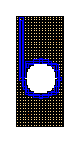
\includegraphics[width=0.24\columnwidth]{icra2018/ip_density_r_3}
%	\caption{Left is an optimal penalty cycle cover. Cycles (blue) cover all areas with high density. After three applications of the tour constraints, a single cycle remains (right). In the intermediate solutions, the subcycles first try to evade the new constraints by reshaping. The final tour omits two of the small hotspots because the cost of integrating them into the single 
%tour is prohibitively expensive.}
%\vspace{-1em}
%	\label{fig:ipexample}
%\end{figure}

\section[Experiments]{Experiments}

The results for representative flights are described below. Figure \ref{fig:fountain} compares the energy consumption for three coverage schemes for a region including a large obstacle in the center.  
A boustrophedon path requires 50 turns, $\SI{187}{\kilo\joule}$, $\SI{160}{\second}$, and $\SI{181}{\metre}$.
A hand-designed path requires 45 turns, $\SI{214}{\kilo\joule}$, $\SI{155}{\second}$, and $\SI{178}{\metre}$.
A path computed using the optimal penalty cycle cover requires only 33 turns, $\SI{184}{\kilo\joule}$, $\SI{133}{\second}$, and $\SI{176}{\metre}$.

\begin{figure}[h]
	\begin{center}
	\includegraphics[width=.48\columnwidth]{icra2018/energy_path_2-notype3}
	\includegraphics[width=.48\columnwidth]{icra2018/energy_path_3-notype3}
	\includegraphics[width=.48\columnwidth]{icra2018/turncost_180}
	\includegraphics[width=.48\columnwidth]{icra2018/energy_path_1}
	\caption[Fountain]{Paths for an environment surrounding a fountain, which poses an obstacle for the UAV. 
	(Top left) The energy consumption during a real world flight for a boustrophedon path.
	(Top right) The energy consumption during a real world flight for a hand-designed loop path.
	(Bottom left) The optimal penalty cycle cover path.
	(Bottom right) The energy consumption during a real-world flight along the optimal path.} \label{fig:fountain}
	\end{center}
	\vspace{-1em}
\end{figure}


A boustrophedon (back-and-forth) path with \SI{2}{\metre} spacing was generated to cover a region $\SI{120}{\metre} \times \SI{15}{\metre}$ at height $\SI{1.5}{\metre}$.
The path was generated using Mission Planner software from ardupilot.org~\cite{Ardupilot}.

For each trial the UAV took off from a resting position on top of the screen.
Flight began manually, with a piloted takeoff of the UAV. After establishing a stable hover at $\SI{3}{\metre}$, control was switched to the autonomous flight plan.
The pilot monitored the flight with the ability to switch to manual operation in case of potential crashes due to GPS error or hazards in the flight plan.
Mosquito strikes detected by the data logger were verified using a GoPro Hero 4 Silver camera attached at the top of the net, as shown in Fig.~\ref{fig:DroneAndNet}.
At night and twilight, the sparks could be detected both visually and audibly from the recorded video.
During the day, the sparks were loud enough to observe over the audio channel of the videos.

The UAV flew eight missions on this field, covering the same path.
It was mainly flown in the early morning and late afternoon, when mosquito activities are more active.
Three flights were flown at noon and early afternoon to ensure that mosquito activities during these periods were not ignored.
However, only two mosquito strikes were observed during this period.
The path covered is about $\SI{1}{\kilo\metre}$ long and typically takes $\SI{12}{\minute}$.

Over the eight missions on this field, there were a total of 11 mosquito strikes.
Figure \ref{fig:strikemap} shows the mission's flight path and the map of all collected strikes.
The mosquito strikes are concentrated at the north and south ends of the field, where there are more trees.
A density map was generated from the collected strikes' position by representing each strike by a Gaussian distribution with the norm on the strike's location and a $\sigma$ of $\SI{10}{\metre}$.
Figure \ref{fig:densitymap} shows the density map generated by summing these Gaussian distributions.

\begin{figure}
	\centering
	\begin{overpic}[width=1.0\columnwidth]{icra2018/strikeMap.png}\end{overpic}
	\caption{\label{fig:strikemap}
	The UAV's path for flight 3 is in red. Strikes collected along this path are represented by yellow dots.} 
\end{figure}


\begin{figure}
	\centering
	\begin{overpic}[width=1.0\columnwidth]{icra2018/densityMap.pdf}\end{overpic}
	\caption{\label{fig:densitymap} Density map showing mosquito distribution on the field, overlaid by flight path 4 in white. 
	} \vspace{-2em}
\end{figure}

These results not only tell where mosquitoes were but also show where mosquitoes were not.
This is a key difference from stationary traps such as~\cite{chen2014flying,linn2016building}.
Figure~\ref{fig:DroneAndNetOutside} shows the UAV during a dawn flight test near the ocean.    

\begin{figure}
	\centering
	\begin{overpic}[width=1.0\columnwidth]{icra2018/OutdoorMosquitoDrone.jpg}\end{overpic}
	\caption{\label{fig:DroneAndNetOutside}
	The UAV and screen during a flight trial near the ocean.
	} 
\end{figure}


\section{Conclusion and Future Work}\label{sec:conclusion}

This chapter presented an approach for finding optimal tours given turn costs and an energy budget, inspired by a mosquito-killing UAV with limited battery life. 
Initial experiments with the UAV and electrified screen track the location of a mosquito-killing UAV as it patrols a field and maps mosquito kills.  

%Future work
Many refinements to the algorithm could be pursued in future work, including changes to both the mosquito-biasing algorithm and the robot flight simulation.  The model may be expanded to continuous space, three dimensions, and to arbitrary turn angles.  These and other considerations will make a more realistic model for future work.  

Further testing of the multi-copter UAV is indicated and will allow more extensive testing of the robustness and accuracy of the hardware design. New sensors that can identify and detect flying insects~\cite{chen2014flying} may be added to the UAV and enable it to proactively steer toward insect swarms and identify insects in realtime.

The concept may be extended to a non-destructive population survey in which the screen could be replaced with a net and, with appropriate lighting, the camera used to record capture events.  Teams of UAVs could work together to map areas more quickly and, by measuring gradients of the distribution, quickly find large mosquito populations.



%%  links for ICRA 2016, 
%%     to submit https://ras.papercept.net
%%     to test pdf
%%  compress using: gs -sDEVICE=pdfwrite -dCompatibilityLevel=1.4 -dNOPAUSE -dQUIET -dBATCH      -sOutputFile=MosquitoUAVcompressed.pdf MosquitoDroneICRA2018.pdf
%
%\documentclass[letterpaper, 10 pt, conference]{ieeeconf}  % Comment this line out if you need a4paper
%%\documentclass[a4paper, 10pt, conference]{ieeeconf}      % Use this line for a4 paper
%\pdfminorversion=4              % tell pdflatex to generate PDF in version 1.4
%\IEEEoverridecommandlockouts                              % This command is only needed if 
%                                                          % you want to use the \thanks command
%
%\overrideIEEEmargins                                      % Needed to meet printer requirements.
%
%% See the \addtolength command later in the file to balance the column lengths
%% on the last page of the document
%
%% The following packages can be found on http:\\www.ctan.org
%%\usepackage{graphics} % for pdf, bitmapped graphics files
%%\usepackage{epsfig} % for postscript graphics files
%%\usepackage{mathptmx} % assumes new font selection scheme installed
%%\usepackage{times} % assumes new font selection scheme installed
%%\usepackage{amsmath} % assumes amsmath package installed
%\usepackage{amssymb}  % assumes amsmath package installed
%\usepackage{mathtools,cuted}
%\usepackage{overpic}
%\graphicspath{{./pictures/},{./pictures/pdf/},{./pictures/ps/},{./pictures/png/},{./pictures/jpg/}}
%\usepackage{amsmath}
%\usepackage[table,xcdraw]{xcolor}
%\usepackage[hidelinks]{hyperref}
%\usepackage{flushend}
%\newcommand{\todo}[1]{\vspace{5 mm}\par \noindent \framebox{\begin{minipage}[c]{0.98 \columnwidth} \ttfamily\flushleft \textcolor{red}{#1}\end{minipage}}\vspace{5 mm}\par}
%
%%units
%\usepackage[per-mode=symbol, detect-weight=true, binary-units=true]{siunitx}
%
%\title{\LARGE \bf
%Using a UAV for Destructive Surveys of Mosquito Population
%}
%
%
%\author{An Nguyen, Dominik~Krupke, Mary Burbage, Shriya Bhatnagar, S{\'a}ndor~P.~Fekete, and Aaron T. Becker% <-this % stops a space
%\thanks{*This work was supported by the National Science Foundation under Grant No.\ \href{http://nsf.gov/awardsearch/showAward?AWD_ID=1553063}{ [IIS-1553063]} and \href{https://nsf.gov/awardsearch/showAward?AWD_ID=1646607}{[IIS-1646607]}.}
%\thanks{A. Nguyen, M. Burbage, S. Bhatnagar, and A. Becker are with the ECE Department at the University of Houston, TX.
%        \protect\url{an.nguyen.vn@ieee.org, atbecker@uh.edu}.
%        S.~Fekete and D.~Krupke are with the Dept.~of Computer Science, TU Braunschweig, Germany,
%      \protect\url{s.fekete@tu-bs.de, d.krupke@tu-bs.de  }
%        }%
%}
%
%\begin{document}
%
%\maketitle
%\thispagestyle{empty}
%\pagestyle{empty}
%
%
%%%%%%%%%%%%%%%%%%%%%%%%%%%%%%%%%%%%%%%%%%%%%%%%%%%%%%%%%%%%%%%%%%%%%%%%%%%%%%%%%
%\begin{abstract}
%This paper introduces techniques for mosquito population surveys in the field using electrified screens (bug zappers) mounted to a UAV. Instrumentation on the UAV logs the UAV path and the GPS location, altitude, and time of each mosquito elimination. 
%Hardware experiments with a UAV equipped with an electrified screen provide real-time measurements of (former) mosquito locations and mosquito-free volumes.
%Planning a trajectory for the UAV that maximizes the number of mosquito kills is related to the Traveling Salesman Problem, the Lawn Mower Problem and, most closely, Milling with Turn Cost. 
%We reduce this problem to considering variants of covering a grid graph with minimum turn cost, corresponding
%to optimized energy consumption. 
%We describe an exact method based on Integer Programming that is able to compute provably optimal instances with over 1,500 pixels. 
%These solutions are then implemented on the UAV.
%\end{abstract}
%
%%%%%%%%%%%%%%%%%%%%%%%%%%%%%%%%%%%%%%%%%%%%%%%%%%%%%%%%%%%%%%%%%%%%%%%%%%%%%%%%%
%
%
%\section{Introduction}
%
%Mosquito-borne diseases kill millions of humans each year~\cite{murray2012global}. 
% Because of this threat, governments worldwide track mosquito populations.
% Tracking individual mosquitoes is difficult because of their small size, wide-ranging flight, and preference for low-light.
% Tracking studies of individual mosquitos have chosen to use small ($\SI{1.2}{\metre} \times \SI{2.4}{\metre}$) indoor regions~\cite{parker2015infrared}, or mating swarms backlit against a solid background~\cite{butail20113d}.
%
%The dominant tools for tracking mosquito populations are stationary traps that are checked at weekly intervals (\textit{e.g.} Encephalitis Vector Surveillance traps and/or gravid traps~\cite{williams2007comparison}). 
%Recent research has focused on making these traps smaller, cheaper, and capable of providing real-time data~\cite{chen2014flying,linn2016building}; however, they still rely on attracting mosquitoes to the trap. 
% This paper presents an alternate solution using an electrified bug-zapping screen mounted on an unmanned aerial vehicle (UAV) as shown in Fig.~\ref{fig:DroneAndNet} to seek out the mosquitoes in their habitat.  As the UAV follows a path, it sweeps out a volume of air, temporarily removing all the mosquitoes in this volume.  By monitoring the voltage across this screen, we can track individual mosquito contacts.
%     UAVs have strict energy budgets, so optimized flight patterns are of crucial importance. As a consequence, putting
%the UAV to good use requires
%methods for computing trajectories that minimize energy consumption along the way, but maximize the total volume of mosquitoes 
%at visited locations.
%
%%the available flight time depends on the flight pattern, as making it crucial to optimize the used trajectories. As it turns out, threquires the utility of a which makes it necessary to  which limit the flight time to a maximum denoted by $T$.
%    %The goal is to design a trajectory for the mosquito screen with duration less than $T$ that maximizes the number of mosquito eliminations.
%
%  \begin{figure}
%\centering
%\begin{overpic}[width=1\columnwidth]{DroneAndNet_v2.pdf}\end{overpic}
%\caption{\label{fig:DroneAndNet}
%	  A hexacopter UAV carrying a $\SI{48}{\centi\metre} \times \SI{61}{\centi\metre}$ rectangular bug-zapping screen. An onboard micro controller monitors the voltage across the screen and records the time, GPS location, humidity, and altitude for each mosquito strike.  At right are three frames recorded by the onboard camera showing mosquito hits, during the day (top) and at twilight.
%See attachment for videos of flight experiments~\cite{Bhatnagar2018}.
%%Video is available at \href{https://youtu.be/1gvJ-yTf-E8}{https://youtu.be/1gvJ-yTf-E8}~\cite{DroneVideo}. 
%\vspace{-2em}
%}
%\end{figure}
%
%
%   % This process can be modeled as sampling without replacement from a point cloud of mobile particles using a mobile agent.  The point cloud particles are generated from a known or unknown distribution, and the mobile agent clears all particles in a swept-out region each time step. 
%%    UAVs have strict energy budgets, which limit the flight time to a maximum denoted by $T$.
%%    The goal is to design a trajectory for the mosquito screen with duration less than $T$ that maximizes the number of mosquito eliminations.%, in probability, samples the most particles.  
%%   We assume the agent can detect each particle collision and can use these detections to modify a planned trajectory.
%%    This paper presents both open-loop trajectories and policies with feedback. 
%%  
%%      \subsection{Overview}
%%A multimedia introduction to the techniques used in this paper is available at~\cite{becker2017zapping}.
%  This paper is arranged as follows.  
%  After a review of related work in \S \ref{sec:relatedWork}, 
%  we describe a design and rationale for a UAV with bug zapper in \S  \ref{Sec:HardwareDesign}.
%    We next present a path planning optimization strategy in   \S \ref{sec:Simulation}.
%  We then describe hardware experiments with the UAV  in \S  \ref{sec:Experiments} and conclude with directions for future research  in \S  \ref{sec:conclusion}.
%  
%  
% 
%
%%%%%%%%%%%%%%%%%%%%%%%%%%%%%%
%  \section{Related Work}\label{sec:relatedWork}
%%%%%%%%%%%%%%%%%%%%%%%%%%%%%%  
%  \noindent \emph{Robotic Coverage}: 
%    Robotic coverage has a long history. The basic problem is one of designing a path for a robot that ensures the robot visits within $r$ distance of every point on the workspace.  For an overview see~\cite{Choset2001}.  This work has been extended to use multiple coverage robots in a variety of ways, including using simple behaviors for the robots~\cite{spears2006physics,Koenig2001}.
%%This is closely related to the art gallery problem~\cite{lee1986computational} but with limited range of visibility.
% %   The key difference in the mosquito coverage problem is that the mosquitoes can move, recontaminating an area previously cleared. We instead have a probability of coverage, as in~\cite{Das2011}.  
%    
%\noindent  \emph{Mosquito Control Solutions}:
%	Mosquito control also has a long history of efforts associated both with monitoring mosquito populations~\cite{dennett2007associations} and with eliminating mosquitoes.  The work involves both draining potential breeding grounds and destroying living mosquitoes~\cite{peter2005tick}.  An array of insecticidal compounds has been used with different application methods, concentrations, and quantities, including both larvicides and compounds directed at adult mosquitoes~\cite{larvicides2005guidelines}.
%	
%	Various traps have been designed to capture and/or kill mosquitoes with increasing sophistication in imitating human bait, as designers strive to achieve a trap that can rival the attraction of a live human~\cite{maliti2015development}.  In recent history, methods have also included genetically modifying mosquitoes so that they either cannot reproduce effectively or cannot transmit diseases successfully~\cite{marshall2009malaria}, and with the recent genomic mapping of mosquito species, new ideas for more targeted work have been formulated~\cite{hill2005arthropod}.
%	
%	Popular methods to control mosquitoes such as insecticides are effective, but they have the potential to introduce long-term environmental damage and mosquitoes have demonstrated the ability to become resistant to pesticides~\cite{ndiath2012resistance}. Traditional electrified screens (bug zappers) use UV light to attract pests but have a large bycatch of non-pest insects~\cite{University-Of-Florida1997}. 
%%	This paper introduces techniques using bug zappers mounted on unmanned vehicles to autonomously seek %out and eliminate mosquitoes in their breeding grounds and swarms. Instrumentation on the bug zappers %logs the GPS location, altitude, weather details, and time of each mosquito hit.  Mosquito control %offices can use this information to analyze the insects' activities. The device can be mounted on a %remote-controlled or autonomous unmanned vehicle. If autonomous, the vehicle can use the data collected %from the electrified screen as feedback to improve the effectiveness of the motion plan. 
%	
%  \noindent  \emph{Robotic Pest Management}:
%As GPS technology has flourished and data processing has become cheaper and more readily available, researchers have explored options for implementing the new technologies in breeding ground removal~\cite{anupa2014identification} and more effective insecticide dispersion~\cite{hur2015low}.  Low-cost UAVs for residential spraying are under development~\cite{amenyo2014medizdroids}.  Even optical solutions have been considered, including laser containment~\cite{boonsri2012laser} or, by extension, exclusion and laser tracking and extermination~\cite{kare2010build}.
%    
%   
%    
%  \section{Hardware Design}\label{Sec:HardwareDesign}%%%%%%%%%%%%%%%%%%
%  %%%%%%%%%%%%%%%%%%%%%%%%%%%%%%%%%%%%%%%
%  This section examines the components of the mosquito UAV system, shown in Fig.~\ref{fig:DroneAndNet}. This includes the UAV, electrified screen, surveying electronics, and a discussion of the energy budget. 
% % The design for the mosquito UAV system been assigned a U.S.\ Provisional Patent Application~\cite{Becker2016patentapp}.
%  
%  \subsection{UAV}
%  
%The UAV is a custom-built, $\SI{177}{\centi\metre}$ wingspan hexacopter, controlled by a Pixhawk flight controller running ArduPilot Mega flight software. The UAV has a 3DR GPS module using the UBlox NEO-7 chipset.
%
%  \subsection{Screen Design}
%     The mosquito screen is designed to eliminate high density mosquito populations. 
%  This screen was constructed from two expanded aluminum mesh panels, spaced apart by \SI{3}{\milli\metre} thick ABS grid. 
%   These mesh panels have \SI{12}{\milli\metre} diamond-shaped  openings, and is held taught by nylon bolts around the perimeter.  
%   The bottom mesh panel is offset by half a diamond (6 mm) to the right to ensure all insects greater than 6 mm cannot pass through the net.
%     The top mesh is held at the reference voltage and the bottom mesh is energized to $1.8~kV$ above the reference voltage.
%     
%  The perimeter is reinforced by two sets of \SI{7}{\milli\metre} diameter fiberglass rods that are inset into 3D printed corner fixtures.
%  These rods protect the frame from getting damaged from any side, and allows the UAV to land without damaging the net.
%
%
%Once assembled, the net weighs \SI{0.948}{\kilogram} and has an overall area of \SI{0.194}{\square\metre}, with the spacer occupying \SI{0.0325}{\square\metre}. 
%This makes the effective net area \SI{0.161}{\square\metre}. %, and the total cost of building a net this size is only \$27.44 USD.
%   
%   
%
%  %Design files and build instructions are available at~\cite{Vinh2016BugNet}.
%
%
%  %%%%%%%%%%%%%%%%%%%%%%%
%  \subsection{Screen Location}
% The UAV carries the bug-zapping screen, which is suspended by paracord rope at each corner.  The location of this screen determines the efficacy of the mosquito UAV, measured in mosquitoes detected per second of flight time. The following describes a simplified analysis to optimize the screen location.
%
%For manufacturing ease, the electrified screen is a rectangle with a width of $d_s$. The screen is suspended a distance $h_s$ beneath the UAV flying at height $h_d$.  We chose to suspend the screen beneath the UAV to avoid the weight of the rigid frame that would be required if the screen were above the UAV and because most mosquito species prefer low flight~\cite{gillies1976vertical}.  This screen can be suspended at any desired angle $\theta$ in comparison to horizontal, as shown in Fig.~\ref{fig:DroneConfigs}.
%Two key parameters are the distance $h_s$ and the optimal angle $\theta$.  The goal is to clear the greatest volume of mosquitoes per second, a volume defined by the UAV forward velocity $v_f$ and the cross-sectional area $h_m \times d_s$ cleared by the screen, as shown in Fig.~\ref{fig:AngleVsSpeed}.
%
% To hover, the UAV must push sufficient air down with velocity $v_d$ to apply a force that cancels the pull of gravity.  The UAV and screen combined have mass $m_{d}$ and its cross section can be approximated as a square with a side length of $d_d$.  The mass flow of air through the UAV's propellers is equal to the product of the change in velocity of the air, the density of the air $\rho_a$, and the cross sectional area.
% 
%     \begin{figure}
%\centering
%\begin{overpic}[width=\columnwidth]{DroneConfigs.pdf}\end{overpic}
%\caption{\label{fig:DroneConfigs}
%The UAV suspends a rectangular bug-zapping screen beneath it.  Propwash pushes incoming mosquitoes downwards, and the UAV clears a volume $h_m \times d_s \times v_f$ each second. Circles show two mosquitoes at equal time intervals relative to the UAV.} 
%\vspace{-1em}
%\end{figure}
%
%
%We assume that air above the UAV is quiescent, so the change in velocity of the air is $v_d~ \si{\metre\per\second}$.
% \begin{align} \label{eq:forceBalanceForDrone}
% \text{Force gravity} & = \left(\text{mass flow}\right) \cdot \text{air velocity} \nonumber \\
% m_{d} \cdot  g &= (v_d \cdot  \rho_a \cdot  d_d^2 ) \cdot  v_d 
%% \text{kg} \cdot \frac{ \text{m}}{ \text{s}^2}&= \left( \frac{ \text{m}}{\text{s}} \cdot  \frac{ \text{kg}}{\text{m}^3}  \cdot \text{m}^2 \right) \cdot  \frac{ \text{m}}{\text{s}}\nonumber
%\end{align}
%
%Then the required \emph{propwash}, the velocity of air beneath the UAV, for hovering is
% \begin{align} \label{eq:dronePropwash}
%v_d = \sqrt{ \frac{ m_d g}{\rho_a d_d^2} }
%\end{align}
%The flight testing site in Houston, Texas is \SI{15}{\metre} above sea level. At sea level the density of air $\rho_a$ is \SI{1.225}{\kilogram\per\cubic\metre}.
%The UAV and instrumentation combined weigh \SI{5.1}{\kilogram} with a width of \SI{0.75}{\metre}. The acceleration due to gravity is \SI{9.871}{\metre\per\square\second}.  Substituting these values gives $v_d = \SI{8.5}{\metre\per\second}$.
%
%Due to propwash, an initially hovering mosquito will fall when under the UAV at a rate of $v_d$.  Relative to the UAV, the mosquito moves horizontally at a rate of $-v_f$.  As shown in Fig.~\ref{fig:DroneConfigs}, we can extend lines with slope $-v_d/v_f$ from the screen's trailing edge to $h_{\textrm{top}}$ and from the leading edge to $h_{\textrm{bottom}}$.
% \begin{align} \label{eq:ClearedCrossSection}
%h_{\textrm{top}} &= h_d - h_s + \frac{d_s}{2} \sin(\theta) +  \frac{d_d + d_s\cos(\theta)}{2}  \frac{v_d}{v_f} \nonumber \\
%h_{\textrm{bottom}} &= h_d - h_s - \frac{d_s}{2} \sin(\theta) +  \frac{d_d - d_s\cos(\theta)}{2}  \frac{v_d}{v_f}  \nonumber \\
%h_m &= h_{\textrm{top}} - h_{\textrm{bottom}} =  d_s\left(\frac{v_d}{v_f}\cos(\theta) + \sin(\theta) \right)
%\end{align}
%The optimal angle is therefore a function of forward and propwash velocity:
%\begin{align} \label{eq:OptimalScreenAngle}
%\ \theta = \mathrm{ArcTan}\left(\frac{v_f}{v_d}\right)
%\end{align}
%
%To ensure the maximum number of mosquitoes are collected, the screen must be sufficiently far below the UAV $ h_s > \frac{d_s}{2} \sin(\theta) +  \frac{d_d + d_s\cos(\theta)}{2}  \frac{v_d}{v_f}$  and the bottom of the screen must not touch the ground, $ h_d > h_s + \frac{d_s}{2} \sin(\theta) $.
%
%      \begin{figure}
%\centering
%\begin{overpic}[width=\columnwidth]{AngleVsSpeed.pdf}\end{overpic}
%\caption{\label{fig:AngleVsSpeed}
%The volume cleared by a UAV is a function of screen angle $\theta$ and forward velocity $v_f$.  Dotted line shows the optimal angle given in \eqref{eq:OptimalScreenAngle}. } 
%\vspace{-1em}
%\end{figure}
% 
%There are practical limits to $h_s$ as well.  Tests with $h_s > \SI{2}{\metre}$ were abandoned because the long length caused the screen to act as a pendulum, introducing dynamics that made the system difficult to fly.
% 
%Changing the flying height $h_d$ of the UAV will target different mosquito populations because mosquitoes are not distributed uniformly vertically. 
% Gillies and Wilkes demonstrated that different species of mosquitoes prefer to fly at different heights~\cite{gillies1976vertical}. 
% 
%   %%%%%%%%%%%%%%%%%%%%%%%
%   \subsection{Wind Tunnel Verification of Net Angle}
%   
%This section describes experiments run in a wind tunnel to verify the simplified net angle analysis in the previous section. 
%Smoke streaklines were used to visualize the flow of air as it passed by the UAV.
%Due to space constraints in the wind tunnel, a free-flying phantom 4 was used instead of the hexacopter used for carrying the zapper. 
%The wind tunnel was set to a \SI{3}{\metre\per\second} flow speed, and the UAV manually flown in approximately stable hovering.
%The solo UAV is \num{0.3} $\times$ \num{0.3} $\times$ \SI{0.2}{\metre}.  The windtunnel has a \SI{1}{\metre} $\times$ \SI{1}{\metre} cross section. 
%%??? brand name of the smoking apparatus?
%As seen from Fig.~\ref{fig:WindTunnel}, the proposed screen position captures free flowing air and air entrained by the UAV propellers.
%This test encouraged us to mount the net as close to the UAV as possible, so that air, and flying mosquitos, entrained by the propellers are pushed into the net.
% 
%
%\begin{figure}
%\centering
%\begin{overpic}[width=1.0\columnwidth]{WindTunnelv01lowres.pdf}\end{overpic}
%\caption{\label{fig:WindTunnel}
%	Frames from wind tunnel test with free-flying UAV at \SI{3}{\metre\per\second} windspeed with smoke for streaklines~\cite{Bhatnagar2018}.  As shown in the frames at right, the proposed screen position (in red) captures free flowing air and air entrained by the UAV propellers.
%	Each black square is \SI{25.4}{\milli\metre} in width.
%  } \vspace{-1em}
%\end{figure}
% 
%
%  %%%%%%%%%%%%%%%%%%%%%%%
%   \subsection{Data Logger}
%   
%   The electrical detection and logging system is powered by a $9~V$ lithium ion battery applied directly to the controller and two AA $3~V$ lithium ion batteries applied to the power circuit for the screen.
%   The controller uses a GPS shield for monitoring the location and altitude as well as a real time clock to timestamp each data point collected from the system.
%   A Raspberry Pi 3 is used for data logging, 
%       sensors include a GPS sensor (NEO-6M Ublox), 
%      a capacitive humidity sensor, a thermistor (DHT22),
%   %ADS1115 16-bit ADC for monitoring the supply-side voltage of the net, and 
%   and an INA219 high side, 12-bit DC current sensor for monitoring the supply-side current delivered to the net.
%   The net current draw is logged at 100 Hz, while GPS and weather sensor data is logged at 1Hz.  
%   All data is stored on an onboard SD card.
%
%  %%%%%%%%%%%%%%%%%%%%%%%
%  \subsection{Energy Budget}
%  
%                  \begin{figure}
%\centering
%\begin{overpic}[width=1.0\columnwidth]{OscilloscopeTrace.pdf}\end{overpic}
%\caption{\label{fig:BugZapTrace}
%					  Current, voltage, and power traces for five \textit{Culex quinquefasciatus} mosquitoes as each contacts the bug-zapping screen at $t=0$.  Contact causes a brief short that recovers in $\SI{160}{\milli\second}$.
%  } 
%  \vspace{-1em}
%\end{figure}
% % \todo{what is the new energy usage of the screen?}
%  
%  
%  Tests with an oscilloscope show that in the steady state, a $\SI{30.5}{\centi\metre} \times \SI{61}{\centi\metre}$ screen and electronics have a power consumption of \SI{3.6}{\watt}.  During a zap, the screen voltage monitoring circuit shorts briefly when the mosquito contacts the screen.  Figure~\ref{fig:BugZapTrace} shows the time sequences for battery and screen voltages, current, and power during five mosquito zaps.  
%% % WE COULD NOT JUSTIFY THIS EQUATION 
%%%  The initial current spike recovery can be modeled with an exponential fit.
%%%
%% \begin{align} \label{eq:BugZapFit}
%%i=69.1e^{-2.7\times10^4 t} ~A
%%\end{align}
%%%
%%The fit in \eqref{eq:BugZapFit} gives a time constant of $36~\mu s$ for the short and a recovery time of $80~\mu s$. 
% Multiplying voltage by current to find the instantaneous power ($p=iv$) and integrating the area under the power curve show a total energy consumption of \SI{4.2}{\milli\joule} for each zap.  Recharging the screen requires more power and is represented in the latter part of the curves.  The overall recovery time is about $\SI{160}{\milli\second}$.  Most of the energy is consumed charging and maintaining the charge on the screen rather than in zapping the mosquitoes.
%  
%  
%
%
%
%%Data
%%The files used for this run of simulations are as follows:
%%MosquitoFlightSimv2p0.m
%%MosquitoSimv2p2randombounce.m
%%MosquitoSimv2p2boustrophedon.m
%%MosquitoSimComparev1p0.m
%%
%%All are located in the Dropbox code folder.
%%Raw data are located in the Excel file Simulation Results.xlsx.
%%    
%    
%%%%%%%%%%%%%%%%%%%
%%%%%%%%%%%%%%%%%%%%%%%%%%%%%%%%%%%%%%% 
\section[Path Planning]{Planning minimal turn cost paths}
%%%%%%%%%%%%%%%%%%%%%%%%%%%%%  

\newcommand{\revised}[1]{{\color{red}#1}}

%The following section present an overview of the algorithm used in the paper's research, which was done by our collaborators in Germany:
%D. Krupke and S.P. Fekete of TU Braunsweig.

\subsection{Modelling mosquito density}
\label{subsec:modelling}
Due to a-priori knowledge of mosquitos' preferred habitats from entomology, we can model the density of mosqitos in a field we want to cover.
This knowledge will help us plan the most efficient path, killing the most mosquitos with the least amount of energy used.
First, we divide a field for coverage into a pixel grid, the size of each pixel dictated by the size of the net and the resoultion of the UAV's GPS.
Each pixel $p_i\in P$ we give a relative density value $c(p_i)$ that describes the estimated mosquito density based on the environmental factor of the pixel.
In $P$ there will only be a subet with high relative density value.
The goal is to maximize the density covered by the set $S\subseteq P$ of visited pixels i.e., $\max_{S\subseteq P} \sum_{p_i\in S} c(p_i)$ within the available battery capacity.
This could be done in one single trip or over multiple trips with multiple batteries.

%The data on the distribution of mosquitoes is given for a two-dimensional grid environment; the grid size
%is induced by the size of the screen, the available data and the desired resolution of the extracted map. 
%For each pixel $p_i\in P$, we are given a relative value
%$c(p_i)$ that describes the estimated a-priori density of mosquitoes, based on data obtained from boustrophedon (back and forth) scans of the area by the UAV;
%this implies that only a subset of pixels carry a significant value.
%Visiting one of the pixels corresponds to sampling and mapping the actual density distribution of mosquitoes. 
%For a dense distribution of mosquitoes
%(which is the case for the instances relevant for pest control), multiple visits to the same pixel do not contribute additional
%knowledge. As a consequence, the objective is to maximize the sampling value of the set $S\subseteq P$ of visited pixels, 
%i.e., $\max_{S\subseteq P} \sum_{p_i\in S} c(p_i)$ {within the available battery capacity}; this may be over the course of a single closed trajectory, or over
%a combination of multiple roundtrips. 

\subsection{Turn cost}

\begin{figure}[h]
\begin{center}
\includegraphics[width=.75\columnwidth]{icra2018/turncost}
\caption[Mosquito hunting drone]{Turns are expensive. See our related video at
\url{https://youtu.be/SFyOMDgdNao} for details, and
\cite{becker2017zapping} for an accompanying abstract.} \label{fig:turncost}
\end{center}
\vspace{-1em}
\end{figure}

UAVs can make turns on the spot, without curvature constraints like a fix-winged aircraft.
However, UAVs turns are energtically expensive.
As Fig.~\ref{fig:turncost} shows, the energy required per meter of travel in a turn is 4 to 5 times as expensive as traveling through a straight path.
The limiting factor for a UAV's flight is its battery capacity, therefor it is important to limit the amount of turns needed per flight while maximizing the amount of pixels visited.
To consider the total energy cost of a turn, we need to limit the types of turns the UAV made.
We consider only strict set of \ang{90} and \ang{180} turns since the UAV does not have minimal turn curvature.
Additionally, the two turn angles allow us to fly around most large obstacles while visiting the pixels around it.

%Planning good trajectories for a UAV is not subject to the same curvature constraints of an ordinary aircraft
%because UAVs can turn on the spot. However, turns are a critical aspect of path
%planning due to their impact on energy consumption.  Battery capacity is {\em the} limiting factor for  UAV flight time. As shown in Fig.~\ref{fig:turncost}, 
%the power output for a desired trajectory is non-uniform.  Flying along a straight path
%is relatively inexpensive but turning is energy intensive. 

%As a consequence, we must consider the total turn costs associated
%with changing direction, as measured by the turn angle.
%As we are not limited by trajectory curvature, we refer to straight-line connections and a finite set of $2\omega$ different
%headings for visiting vertices. For the most natural case of orthogonal grids $\omega=2$. When
%surveying non-isolated mosquito hotspots (whose size greatly exceeds the size of the UAV), we are not dealing with
%isolated pixels and the modeling error of this restriction is small.

%TODO: I guess one can save space here by e.g. skipping subset cover.
%Now we consider different trajectory types.
%A {\em cycle} is a roundtrip of a subset $S\subseteq P$ that visits all points in $S$ and returns to the origin, a {\em cycle cover} of $P$ is a set of cycles
%that together visit all points in $P$, and a {\em tour} is a single cycle that visits all points in $P$. A {\em subset cycle cover} for $S\subset P$ is a cycle
%cover that covers at least the points in $S$, while a {\em subset tour} is a tour of at least the points in $S$. For any of these structures, we are interested in
%%cycle covers or tours of {\em minimum total turn cost}. 
%{cycle covers or tours of {\em minimum total travel cost}. 
%The travel/battery cost is a linear combination of the number of pixel transitions (distance) and the weighted number of turns, 
%corresponding to the total turn angle.
%}
%In addition, a {\em minimum turn-cost penalty cycle cover}  or a {\em minimum turn-cost penalty tour}
%visits a subset $R\subset P$, such that the sum of total travel cost and the sum $\sum_{i\not\in R} c(p_i)$ of values of 
%unvisited pixels is minimized. 
%The travel/battery cost is a linear combination of the number of pixel transitions (distance) and the weighted number of turns, 
%corresponding to the total turn angle.
%Note that the travel cost
%may be a linear combination of turn and travel cost, as long as triangle inequality is satisfied.

%\subsection{Computational Complexity}
%\label{subsec:complexity}
%Finding optimal covering paths that map a given region is closely related to the famous 
%\emph{Traveling Salesman Problem (TSP)}, which asks to minimize
%total length of a single tour that covers all of a given set of locations. The TSP is one of 
%the classic NP-hard problems, so we cannot expect a general method that finds
%a provably optimal solution for any  instance in polynomially bounded time.
%A generalization of the TSP is
%the \emph{Lawnmower Problem} (see Arkin et al.~\cite{arkin2000approximation}, which considers coverage by
%a tool of nontrivial size. For the objective of minimizing the total cost (in particular, the turn
%cost), Arkin et al.~\cite{arkin2005optimal} showed that finding minimum-turn tours in grid graphs is NP-hard,
%even if a minimum-turn cycle cover is given. The complexity of finding a set of multiple cycles that cover a 
%given set of locations at minimum total turn cost had remained elusive for many years; \emph{Problem~{53}} in \emph{The Open Problems Project}
%%edited by Demaine, Mitchell, and O'Rourke~\cite{openproblemproject}
%asks for the complexity of finding a minimum-cost (full) cycle cover in a 2-dimensional grid graph. This is not 
%obvious: large parts of a solution can usually easily be deduced by local information and 2-factor techniques.
%Arkin et al. showed~\cite{arkin2005optimal,arkin2001optimal} that the full coverage variant in {\em thin} grid graphs (which do not contain a $2\times 2$ square,
%so every pixel is a boundary pixel) is solvable in polynomial time. In separate work~\cite{dom3}, two of us were able to resolve this
%issue by showing that finding a cycle cover of minimum turn cost is  NP-hard.

%\subsection{Mathematical Optimization}
%\label{subsec:complexity}
%A powerful approach for finding optimal solutions to instances of NP-hard problems is the use
%of Integer Programming (IP). While solving an IP still requires exponential time in the worst case,
%using carefully crafted mathematical models in combination with specific algorithm engineering and available
%IP solvers enables solving instances of considerable size to provable optimality.
%For our purposes, we can describe the problem as follows. 
%
%\paragraph{Penalty Cycle Covers}
%The set $P$ of pixels corresponds to a given grid graph $G(P,E)$ in which each pixel $p_j\in P$ is adjacent to the set $N(p_j)$
%of pixels in $P$ that share an edge with $p_j$.
%Each vertex $p_j\in P$ has a scalar reward $c(p_j)$ for visiting (or penalty for not visiting), 
%and a function $\text{cost}_j(i,k)\in \mathbb{Z}^+_0$  that maps the cost of traveling from $p_i$ to $p_j$ to $p_k$, where  $p_i,p_k\in N(p_j)$ are adjacent pixels to   $p_j$.
%This cost is symmetric, i.e. $\text{cost}_j(i,k)=\text{cost}_j(k,i)$. %TODO: Or cost(ijk) or cost(i,j,k) or cost(p_i, p_j, p_k)
%The integer program uses two types of variables: integer variables
%$x_{ijk}=x_{kji}$ that state how often passage $p_i-p_j-p_k$ or $p_k-p_j-p_i$ is used and
%Boolean variables $y_{j}$ that indicate that the pixel $p_j\in V$ is not covered,
%i.e., the penalty is paid.  This results in the following formulation: 
%%IP Formulation TODO
%%\begin{strip}
%%\begin{eqnarray}
%%	\min & \displaystyle  \sum_{p_j\in P} \sum_{p_i,p_k\in N(p_j)} \text{cost}_j(i,k) \cdot x_{ijk} + \sum_{p_j\in P}c(p_j) \cdot y_j\label{eq:obj}\\
%%	\text{s.t.}			& 1\leq\displaystyle 4 \cdot y_j +\sum_{p_i,p_k\in N(p_j)} x_{ijk} \leq 4&\forall p_j\in P \label{eq:ip:constr1}\\
%%						& \displaystyle 2 \cdot x_{jij} +\sum_{p_k\in N(p_i), p_k\not= p_j}x_{jik} = 2 \cdot x_{iji}+\sum_{p_k\in N(p_j), p_k\not= p_i}x_{ijk}  & \forall \{p_i,p_j\}\in E \label{eq:ip:constr2}\\
%%						& x_{ijk}\in\mathbb{N}_0, y_j\in \mathbb{B} & \forall p_j\in P, \{p_i,p_k\}\subseteq N(p_j)
%%\end{eqnarray}
%%\end{strip}
%\begin{eqnarray}
%	\min  \displaystyle  \sum_{p_j\in P} \sum_{p_i,p_k\in N(p_j)} \text{cost}_j(i,k) \cdot x_{ijk} + \sum_{p_j\in P}c(p_j) \cdot y_j\label{eq:obj}
%\end{eqnarray}
%with constraints
%\begin{eqnarray}
%	 1\leq\displaystyle 4 \cdot y_j +\sum_{p_i,p_k\in N(p_j)} x_{ijk} \leq 4, &\forall p_j\in P \label{eq:ip:constr1}
%\end{eqnarray}
%\begin{eqnarray}	
%%	\displaystyle  x_{jij}   \underset{ p_k\in N(p_i), p_k\not = p_j}{+ \tfrac{1}{2}\sum x_{jik}}  \!\!    =   x_{iji}      \underset{p_k\in N(p_j), p_k\not= p_i}{+ \tfrac{1}{2}\sum x_{ijk}},  & \forall \{p_i,p_j\}\in E 
%	\displaystyle 2 x_{jij}  \!\!\!   \underset{ p_k\in N(p_i), p_k\not = p_j}{+\sum x_{jik}}  \!\!\!\!\!    = 2  x_{iji} \!\!\!     \underset{p_k\in N(p_j), p_k\not= p_i}{+\sum x_{ijk}},  & \forall \{p_i,p_j\}\in E \label{eq:ip:constr2}
%\end{eqnarray}
%\begin{eqnarray}	
%	 x_{ijk}\in\mathbb{N}_0, y_j\in \mathbb{B} ,& \forall p_j\in P, \{p_i,p_k\}\subseteq N(p_j)  \label{eq:ip:constrINTS}
%\end{eqnarray}
%
%
%%Describe IP
%The objective function in Eq.~\ref{eq:obj} minimizes the total cost of the cycles and the uncovered pixels.
%Eq.~\ref{eq:ip:constr1} enforces a pixel to be covered or the \emph{not covered} variable to be set to {\tt true}.
%Arkin et al.~\cite{arkin2005optimal} showed that no pixel needs to be visited more than four times, otherwise a simple local optimization 
%can be performed.
%Eq.~\ref{eq:ip:constr2} enforces the transitions between two adjacent pixels to match.
%Eq.~\ref{eq:ip:constrINTS} enforces that the variables are integers or booleans.
%
%We can solve a wide spectrum of instances with different kinds of probability distributions up to a size of 
%$1500$ pixels to provable optimality.  
%Optimal solutions for different densities scalings of an instance with $1783$ pixels are shown in Fig.~\ref{fig:ip:differentdensities}. 
%To solve larger instances the optimality constraint can be relaxed or the grid graph can be split and 
%the subgraphs solved separately.
%\begin{figure}
%	\centering
%	\includegraphics[width=0.32\columnwidth]{icra2018/ip_density_cc_2}
%	\includegraphics[width=0.32\columnwidth]{icra2018/ip_density_cc_4}
%	\includegraphics[width=0.32\columnwidth]{icra2018/ip_density_cc_8}
%	\caption{Optimal cycle covers with different density scaling. The middle has twice and the right instance has four times the density as the left. {In these instances, the cost of a $90^\circ$ is five times that of a straight pixel transition.}}
%	\label{fig:ip:differentdensities}
%	%TODO: this picture can be removed if the paper is too long.
%	\vspace{-1em}
%\end{figure}
%
%\paragraph{Tours}
%Computing a minimum cycle cover may result in several subcycles that need to be visited separately, which is appropriate
%for the use of several UAVs or when several separate roundtrips by the same UAV are convenient.
%If we want to determine connected roundtrips by a single UAV, we need to connect the components of
%a cycle cover to a tour. This can be achieved via integer programming by adding additional constraints for
%separating these {\em subtours}.
%
%%Separation constraints
%This separation of subtours is more complicated than for the classic TSP because there may be tours that 
%cross but are not connected. Instead of connecting two subtours, one subtour can also be discarded.
%
%% Second constraint is sufficient but inefficient because it cannot efficiently force to distant subtours to connect.
%We first consider a constraint (Eq.~\ref{eq:gg:fc:ip1:subcycle:2}) that is able to separate any given solution with multiple subtours.
%Let $Q$ be the pixels of a selected subtour. 
%Let $p_\ell\in Q$ be a pixel with high density and no other subtours crossing it
%%(if this is not possible, one can assume the subtours covering this field to be
%%connected), 
%and $p_{\ell'}\not\in Q$ be another covered pixel with high density.
%These two pixels are used for `defusing': if one of them is no longer covered, the constraint is automatically fulfilled.
%We denote by $Q_s$ the pixels that are covered only by straight paths in the subtour.
%%We denote by $Q_s$ the pixels that are covered only straight by the subtour.
%$T(p_j)$ describes the turn variables of a pixel $p_j$.
%$x'$ refers to the variable assignment in the current solution.
%%\begin{strip}
%%\begin{equation}
%%	y_{\ell}+y_{\ell'}+\sum_{p_i,p_k\in N(p_\ell), x'_{i\ell k}=0} x_{i\ell k} + \sum_{t\in T(v), v\in Q_s-p_\ell} t + \sum_{ p_j\in Q\setminus (Q_s+p_\ell), p_i\not=p_k\in N(p_j), x'_{ijk}=0} x_{ijk} \geq 1 \label{eq:gg:fc:ip1:subcycle:2}
%%\end{equation}
%%\end{strip}
%\begin{align}
%	1 \leq y_{\ell} &+y_{\ell'}+\sum_{p_i,p_k\in N(p_\ell), x'_{i\ell k}=0} x_{i\ell k}  + \sum_{t\in T(v), v\in Q_s-p_\ell} t \nonumber \\
%	   & + \sum_{ p_j\in Q\setminus (Q_s+p_\ell), p_i\not=p_k\in N(p_j), x'_{ijk}=0} x_{ijk} \label{eq:gg:fc:ip1:subcycle:2}
%\end{align}
%
%
%While this constraint suffices for capturing the mathematical conditions, its practical performance is unsatisfactory
%for connecting distant subtours. A better approach is described in the following;
%this is not always sufficient but more efficient in connecting distant cycles. 
%We use the same definitions as for the previous constraint, but consider an additional set $Q'$ that is a superset of $Q$.
%$Q$ are the pixels of a subtour and $p_{\ell}$ is a valuable pixel. $Q'$ is a superset of $Q$ (possibly equal to $Q$). $p_{\ell'}$ is a valuable
%pixel outside of $Q'$. 
%The constraint enforces that either $p_{\ell}$ or $p_{\ell'}$ is uncovered, or there is a path on 
%the margin of $Q'$ that connects $p_{\ell}$ and $p_{\ell'}$.
%
%\begin{equation}
%	\displaystyle y_{\ell}+y_{\ell'}+\sum\limits_{x\in \text{Leaving}(Q')} x \geq 1
%\end{equation}
%We use two ways to choose $Q'$ for 
%%each of the different 
%{these} subtour elimination constraints:
%	$Q'=Q$ which is similar to the classical TSP constraint or 
%	%\item $Q'$ a sliced of part of the environment (horizontal or vertical cut through the environment). %Not implemented in new implementation.
%	$Q'$ is the Voronoi cell of the subtour. %Voronoi cells of close subtours are merged. %Not in the new implementation but I think this was a good idea. Possibly reimplement it.
%
%\subsection{Computational Results}
%\label{subsec:computational}
%
%\begin{figure}[h]
%	\includegraphics[width=\columnwidth]{icra2018/runtime_cc_optimal_random.pdf}
%	\caption{Runtime of solving benchmark instances to optimality. Shown
%	are the times of ten instances for each size, with a timeout at \SI{900}{\second}, as
%well as the percentage of solved instances. Only the number of turns is minimized in these instances.} \label{fig:experimentsfromthesis}
%\vspace{-1em}
%\end{figure}
%
%We evaluated the effectiveness of our optimization method by testing it on a suite of benchmark instances based on
%random natural grid graphs with random densities; %corresponding to the setting of mosquito distributions,
%the probability of a pixel to be added during test instance generation is correlated with its neighborhood, resulting in smoother boundaries which are more natural than purely random instances.
%% Changed the sentence above. It didn't make any sense to me.
%The tests were carried out for \num{10} instances for each size in the range up to \num{1400} pixels. 
%We used modern desktop computers equipped with an \emph{Intel(R) 
%Core(TM) i7-6700K CPU @ \SI{4.00}{\giga\Hz}} and \SI{64}{\giga\byte} of RAM. The integer programs were computed with CPLEX version 12.5.0.0 
%and the parameters \texttt{EpInt=0}, \texttt{ EpGap=0}, \texttt{ EpOpt=1e-9}, and \texttt{ EpAGap=0}.
%Fig.~\ref{fig:experimentsfromthesis} shows runtimes for solving penalty cycle cover to optimality. 
%Instances that took longer than \SI{15}{\minute} were aborted.
%As shown in the figure, 
%even at \num{1400} pixels we were still able to solve half of the instances to provable optimality.
%Even for the aborted instances, the computed solutions were within a few percentage points of
%the provable lower bound, meaning that they were nearly optimal.
%
%%PC stats, copied from thesis.
%
%Fig.~\ref{fig:ipexample} shows an example of iteratively computing an optimal tour with the described integer program.
%This example took less than a minute of total computing time.
%It assumed that $90^\circ$ turns cost five times as much as a straight pixel transition (distance).
%%but other instances are much more problematic. %such that selecting and connecting a subset of cycles instead of separating the integer program is more practical.
%
%\begin{figure}
%	\includegraphics[width=0.24\columnwidth]{icra2018/ip_density}
%	\includegraphics[width=0.24\columnwidth]{icra2018/ip_density_r_1}
%	\includegraphics[width=0.24\columnwidth]{icra2018/ip_density_r_2}
%	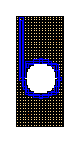
\includegraphics[width=0.24\columnwidth]{icra2018/ip_density_r_3}
%	\caption{Left is an optimal penalty cycle cover. Cycles (blue) cover all areas with high density. After three applications of the tour constraints, a single cycle remains (right). In the intermediate solutions, the subcycles first try to evade the new constraints by reshaping. The final tour omits two of the small hotspots because the cost of integrating them into the single 
%tour is prohibitively expensive.}
%\vspace{-1em}
%	\label{fig:ipexample}
%\end{figure}

%%%%%%%%%%%%%%%%%%%%
%
%    \section{Experiments}\label{sec:Experiments}
%
%The results for representative flights are described below. Figure \ref{fig:fountain} compares the energy consumption for three coverage schemes for a region including a large obstacle in the center.  
%A boustrophedon path requires 50 turns, $\SI{187}{\kilo\joule}$, $\SI{160}{\second}$, and $\SI{181}{\metre}$.
%A hand-designed path requires 45 turns, $\SI{214}{\kilo\joule}$, $\SI{155}{\second}$, and $\SI{178}{\metre}$.
%A path computed using the optimal penalty cycle cover requires only 33 turns, $\SI{184}{\kilo\joule}$, $\SI{133}{\second}$, and $\SI{176}{\metre}$.
%
%\begin{figure}[h]
%\begin{center}
%                \includegraphics[width=.48\columnwidth]{./pictures/energy_path_2-notype3}
%                \includegraphics[width=.48\columnwidth]{./pictures/energy_path_3-notype3}
%                                \includegraphics[width=.48\columnwidth]{./pictures/turncost_180}
%                \includegraphics[width=.48\columnwidth]{./pictures/energy_path_1}
%		\caption[Fountain]{Paths for an environment surrounding a fountain, which poses an obstacle for the UAV. 
%		(Top left) The energy consumption during a real world flight for a boustrophedon path.
%		(Top right) The energy consumption during a real world flight for a hand-designed loop path.
%		(Bottom left) The optimal penalty cycle cover path.
%		(Bottom right) The energy consumption during a real-world flight along the optimal path.} \label{fig:fountain}
%\end{center}
%\vspace{-1em}
%\end{figure}
%
%
%A boustrophedon (back-and-forth) path with \SI{2}{\metre} spacing was generated to cover a region $\SI{120}{\metre} \times \SI{15}{\metre}$ at height $\SI{1.5}{\metre}$.
%The path was generated using Mission Planner software from ardupilot.org~\cite{Ardupilot}.
%
%For each trial the UAV took off from a resting position on top of the screen.
%Flight began manually, with a piloted takeoff of the UAV. After establishing a stable hover at $\SI{3}{\metre}$, control was switched to the autonomous flight plan.
%The pilot monitored the flight with the ability to switch to manual operation in case of potential crashes due to GPS error or hazards in the flight plan.
%Mosquito strikes detected by the data logger were verified using a GoPro Hero 4 Silver camera attached at the top of the net, as shown in Fig.~\ref{fig:DroneAndNet}.
%At night and twilight, the sparks could be detected both visually and audibly from the recorded video.
%During the day, the sparks were loud enough to observe over the audio channel of the videos.
%
%The UAV flew eight missions on this field, covering the same path.
%It was mainly flown in the early morning and late afternoon, when mosquito activities are more active.
%Three flights were flown at noon and early afternoon to ensure that mosquito activities during these periods were not ignored.
%However, only two mosquito strikes were observed during this period.
%The path covered is about $\SI{1}{\kilo\metre}$ long and typically takes $\SI{12}{\minute}$.
%
%Over the eight missions on this field, there were a total of 11 mosquito strikes.
%Figure \ref{fig:strikemap} shows the mission's flight path and the map of all collected strikes.
%The mosquito strikes are concentrated at the north and south ends of the field, where there are more trees.
% A density map was generated from the collected strikes' position by representing each strike by a Gaussian distribution with the norm on the strike's location and a $\sigma$ of $\SI{10}{\metre}$.
%Figure \ref{fig:densitymap} shows the density map generated by summing these Gaussian distributions.
%
%\begin{figure}
%\centering
%\begin{overpic}[width=1.0\columnwidth]{strikeMap.png}\end{overpic}
%\caption{\label{fig:strikemap}
%	The UAV's path for flight 3 is in red. Strikes collected along this path are represented by yellow dots.} 
%\end{figure}
%
%
%\begin{figure}
%\centering
%\begin{overpic}[width=1.0\columnwidth]{densityMap.pdf}\end{overpic}
%\caption{\label{fig:densitymap} Density map showing mosquito distribution on the field, overlaid by flight path 4 in white. 
%    } \vspace{-2em}
%\end{figure}
%
%These results not only tell where mosquitoes were but also show where mosquitoes were not.
%This is a key difference from stationary traps such as~\cite{chen2014flying,linn2016building}.
%Figure~\ref{fig:DroneAndNetOutside} shows the UAV during a dawn flight test near the ocean.    
%
%\begin{figure}
%\centering
%\begin{overpic}[width=1.0\columnwidth]{OutdoorMosquitoDrone.jpg}\end{overpic}
%\caption{\label{fig:DroneAndNetOutside}
%    The UAV and screen during a flight trial near the ocean.
%    } 
%\end{figure}
%
%
%%%%%%%%%%%%%%%%%%%%%%%%%%%%%%
%\section{Conclusion and Future Work}\label{sec:conclusion}
%
%This paper presented an approach for finding optimal tours given turn costs and an energy budget, inspired by a mosquito-killing UAV with limited battery life. 
%Initial experiments with the UAV and electrified screen track the location of a mosquito-killing UAV as it patrols a field and maps mosquito kills.  
%
%%Future work
%Many refinements to the algorithm could be pursued in future work, including changes to both the mosquito-biasing algorithm and the robot flight simulation.  The model may be expanded to continuous space, three dimensions, and to arbitrary turn angles.  These and other considerations will make a more realistic model for future work.  
%
%Further testing of the multi-copter UAV is indicated and will allow more extensive testing of the robustness and accuracy of the hardware design. New sensors that can identify and detect flying insects~\cite{chen2014flying} may be added to the UAV and enable it to proactively steer toward insect swarms and identify insects in realtime.
%
%The concept may be extended to a non-destructive population survey in which the screen could be replaced with a net and, with appropriate lighting, the camera used to record capture events.  Teams of UAVs could work together to map areas more quickly and, by measuring gradients of the distribution, quickly find large mosquito populations.
%
%
%%\section*{ACKNOWLEDGMENT}
%
%\section*{ACKNOWLEDGMENT}
%The authors acknowledge the helpful advice and feedback from Martin Reyna Nava, MS, Medical Entomologist and Technical Operations Manager and Mustapha Debboun, Ph.D, BCE, Director Mosquito Control Division, of the Harris County Public Health \& Environmental Services, Mosquito Control Division.
%%RULES: http://www.nsf.gov/pubs/policydocs/pappguide/nsf16001/aag_6.jsp
%This material is based upon work supported by the National Science Foundation under Grant No.\ 
%\href{https://nsf.gov/awardsearch/showAward?AWD_ID=1553063}{IIS-1553063} and
%\href{https://nsf.gov/awardsearch/showAward?AWD_ID=1646607}{IIS-1646607}.
%%Optional disclaimer (mandatory for non-scientific)
%%Any opinions, findings, and conclusions or recommendations expressed in this material are those of the authors and do not necessarily reflect the views of the National Science Foundation.
%Thank you to Professor Daniel Araya for designing and running the wind tunnel verification tests.
%
%%%%%%%%%%%%%%%%%%%%%%%%%%%%%%%%%%%%%%%%%%%%%%%%%%%%%%%%%%%%%%%%%%%%%%%%%%%%%%%%%
%
%
%\bibliographystyle{IEEEtran}
%\bibliography{./bib/mosquitorefs}%
%
%%\begin{thebibliography}{99}
%%
%%\bibitem{c1} D. V. Maliti, N. J. Govella, G. F. Killeen, N. Mirzai, P. C. D. Johnson Development and evaluation of mosquito-electrocuting traps as alternatives to the human landing catch technique for sampling host-seeking malaria vectors, Malaria Journal, vol. 14:502, Dec. 2015
%%\bibitem{c2} Anupa Elizabeth, P.; Saravana Mohan, M.; Philip Samuel, P.; Pandian, S.R.; Tyagi, B.K.,Identification and eradication of mosquito breeding sites using wireless networking and electromechanical technologies, in Recent Trends in Information Technology (ICRTIT), 2014 International Conference, Chennai, 2014, pp. 1-6.
%%\bibitem{c3} Hur, B.; Eisenstadt, W., Low-power wireless climate monitoring system with RFID security access feature for mosquito and pathogen research, in Mobile and Secure Services (MOBISECSERV), 2015 First Conference, Gainsville, pp.1-5, 20-21 Feb. 2015
%%
%%
%%
%%
%%
%%\end{thebibliography}
%
%
%
%
%\end{document}
